\documentclass[12pt,a4paper]{article}
\usepackage[ngerman]{babel}
\usepackage[utf8]{inputenc}
\usepackage[unicode=true,bookmarks=false,bookmarksopen=true]{hyperref}

\usepackage{xcolor}
\usepackage{graphicx}
\usepackage{tikz}

\usepackage{listings}

\def\checkmark{\tikz\fill[scale=0.4](0,.35) -- (.25,0) -- (1,.7) -- (.25,.15) -- cycle;}

\definecolor{pGreen}{rgb}{0.44, 0.71, 0}
\definecolor{nRed}{rgb}{0.74, 0, 0}

\title{ORES Custom Documentation V}
%\author{Tom Gülenman}
\date{}
\begin{document}
\maketitle
\textit{Disclaimer: No guarantee for the correctness of information / explanations / sources is given.}\\
%
\section*{Goals}
\begin{enumerate}
\item Metric list:
\begin{itemize}
\item Add examples to each metric (if possible)
\item Adjust the description of counts $\rightarrow$ labels, predictions
\end{itemize}
\item Research what form of revision data is needed (for existing visualizations, but also in general) $\rightarrow$ also check RecentChanges and new Filters and what API calls look like in that context
\item Watch \href{https://www.dataschool.io/roc-curves-and-auc-explained}{``ROC curves and Area Under the Curve explained''} and think about what parameters could be used in which ways to filter the output of the current UI (currently: X inputs $\rightarrow$ X outputs)
\begin{description}
\item Also check out: \href{https://www.kaggle.com/general/7517#post41179}{Precision-Recall AUC vs ROC AUC discussion}
\end{description}
\item Read \href{https://doi.org/10.1145/3185517}{A Review of User Interface Design for Interactive Machine Learning} (carefully!)
\item Think about what could be the goal of this thesis
\end{enumerate}
%
%
%
%TODO eigene grafik + google rausnehmen?
\newpage
\section{Crucial metrics: \textbf{damaging}-model}
Metrics simple list:\\

\begin{tabular}{| l | l |}
\hline 
!f1 & \checkmark \\ \hline
!precision & \checkmark \\ \hline
!recall & \checkmark \\ \hline
accuracy & \checkmark \\ \hline
counts & \checkmark \\ \hline
f1 & \checkmark \\ \hline
filter\_rate & \checkmark \\ \hline
fpr & \checkmark \\ \hline
match\_rate & \checkmark \\ \hline
pr\_auc & \checkmark \\ \hline 
precision & \checkmark\\ \hline
rates & \checkmark \\ \hline 
recall &  \checkmark\\ \hline
roc\_auc & \checkmark \\ \hline
\end{tabular}

\begin{description}
\item Again, changes have been made to the list and explanations, compared to the version in oresDoc4. The structure of explanations will be as follows:
\item For each metric (if possible) there will be:
\begin{enumerate}
\item The formula based on the \textbf{confusion matrix}
\item A definition
\item An intuitive explanation with an example
\item Its meaning based on the \textbf{loan threshold} representation by Google (\href{https://research.google.com/bigpicture/attacking-discrimination-in-ml/}{Link})
\end{enumerate}
\end{description}
\subsection*{Explanations: References}
\begin{itemize}
\item Confusion Matrix 
\begin{description}
\item 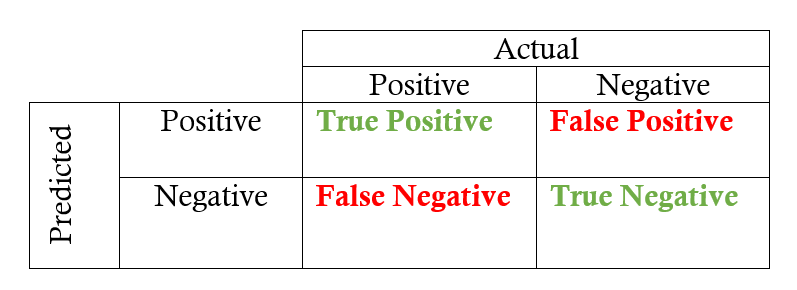
\includegraphics[scale=0.3]{resources/3/confusionMatrix}
\item Abbreviations: \textbf{\textcolor{pGreen}{TP}}, \textbf{\textcolor{nRed}{FP}}, \textbf{\textcolor{nRed}{FN}} and \textbf{\textcolor{pGreen}{TN}}.
\end{description}
\item Loan Threshold
\begin{description}
\item 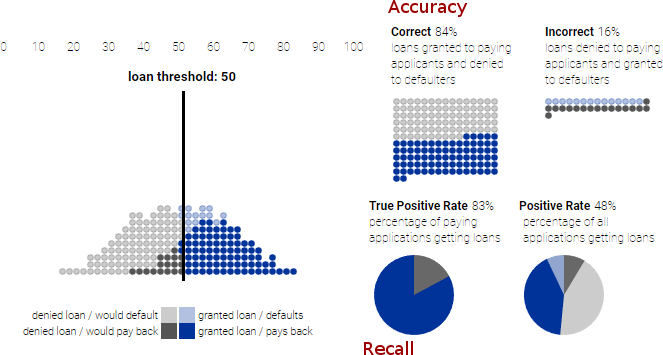
\includegraphics[scale=0.57]{resources/4/loanML4}
\end{description}
\end{itemize}
%
\subsection*{The example scenario}
To ease the understanding, let's stick to the following scenario and refer to it for each metric:
\begin{itemize}
\item 100 people represent our total population
\item 35\% of our population is infected with disease X
\begin{description}
\item That leaves us with the following \textbf{labels}: \textbf{35} \colorbox{pGreen}{\textbf{positives}} and \textbf{65} \colorbox{nRed}{\textbf{negatives}} (being tested for disease X;)
\item 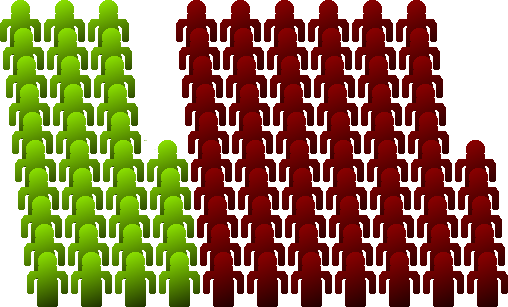
\includegraphics[scale=0.5]{resources/5/exampleBase}
\end{description}
\item A classifier is now supposed to classify every person of our population (based on their visible symptoms for example). This is the \textbf{prediction}:
\begin{itemize}
\item If our algorithm says a person is infected, that person will be classified as a \colorbox{pGreen}{\textbf{positive}}, and marked with radioactive symbol:
\begin{description}
\item 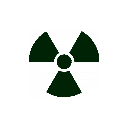
\includegraphics[scale=0.3]{resources/5/radioactive}
\end{description}
\item If the prediction results in a \colorbox{nRed}{\textbf{negative}}, the person will be marked with a sun symbol:
\begin{description}
\item 
\includegraphics[scale=0.3]{resources/5/sun}
\end{description}
\end{itemize}
\item The classifier may predict that:
\begin{itemize}
\item out of the 35 \colorbox{pGreen}{infected people}, \textbf{30} are infected (those 30 are what we call \textbf{true positives}) and \textbf{5} are not (those 5 are \textbf{false negatives}) 
\item out of the 65 \colorbox{nRed}{non infected people}, \textbf{10} are infected (\textbf{false positives}) and \textbf{55} are not (\textbf{true negatives})
\begin{description}
\item 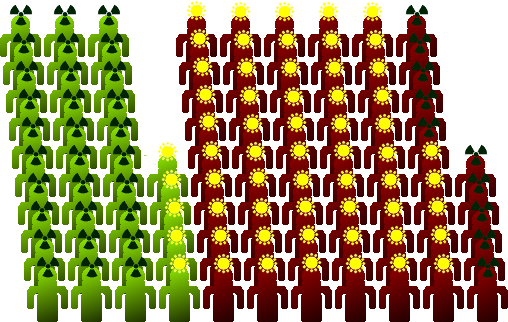
\includegraphics[scale=0.5]{resources/5/examplePredicted}
\item 
\includegraphics[scale=0.5]{resources/5/exampleTP} \textbf{true positive}: infected and correctly predicted
\item 
\includegraphics[scale=0.5]{resources/5/exampleFN} \textbf{false negative}: infected and incorrectly predicted
\item 
\includegraphics[scale=0.5]{resources/5/exampleTN} \textbf{true negative}: not infected and correctly predicted
\item 
\includegraphics[scale=0.5]{resources/5/exampleFP} \textbf{false positive}: not infected and incorrectly predicted
\end{description}
\end{itemize}
\end{itemize}

\paragraph{Let's get started.}
\subsection{recall}
\begin{enumerate}
\item $\frac{\texttt{TP}}{\texttt{TP} + \texttt{FN}}$
\item Recall ($\equiv$ true positive rate $\equiv$ ``sensitivity'') is the ability of a model to find all relevant cases within the dataset.
\item Now, in our example scenario, the relevant cases are the infected people. We absolutely want to identify those: 
\includegraphics[scale=0.3]{resources/5/exampleP}. The ability of the model to identify those depends on how many will be \textbf{correctly} predicted to be infected: 
\includegraphics[scale=0.3]{resources/5/exampleTP}.
\begin{description}
\item In other words, we are looking for the ratio of correctly predicted to be infected people to all infected people.
\item That leads to $\frac{\sum 
\includegraphics[scale=0.3]{resources/5/exampleTP}}{\sum 
\includegraphics[scale=0.3]{resources/5/exampleP}}$, with $
\includegraphics[scale=0.3]{resources/5/exampleP} = 
\includegraphics[scale=0.3]{resources/5/exampleTP} + 
\includegraphics[scale=0.3]{resources/5/exampleFN}$, which is equivalent to the formula in \textbf{1.}, if you replace the symbols with their confusion matrix counterpart according to the legend in \textbf{The example scenario}.
\end{description}
\item $\frac{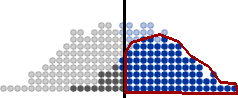
\includegraphics[scale=0.6]{resources/4/loanTP}}{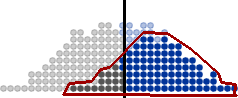
\includegraphics[scale=0.6]{resources/4/loanTP+FN}}$
\end{enumerate}
%
\subsection{precision}
\begin{enumerate}
\item Ability of the model to find only relevant cases within the dataset
\end{enumerate}
\begin{tabular}{|l|l|l|l|}
\hline
2. & 3. & 4.\\ 
$= \frac{\texttt{TP}}{\texttt{TP} + \texttt{FP}}$ & $= \frac{
\includegraphics[scale=0.1]{resources/3/confusionCircleTP}}{
\includegraphics[scale=0.1]{resources/3/confusionCircleTP+FP}}$ & $= \frac{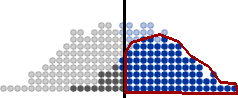
\includegraphics[scale=0.6]{resources/4/loanTP}}{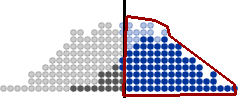
\includegraphics[scale=0.6]{resources/4/loanTP+FP}}$\\ \hline
\end{tabular}
%
\subsection{f1}
\begin{enumerate}
\item F1-Score, the harmonic mean of recall and precision, a metric from 0 (worst) to 1 (best), used to evaluate the accuracy of a model by taking recall and precision into account 
\end{enumerate}
\begin{tabular}{|l|l|l|l|}
\hline
2. & 3. & 4.\\ 
- & - & - \\ \hline
\end{tabular}
\begin{description}
\item $=2*\frac{\texttt{precision} * \texttt{recall}}{\texttt{precision}+\texttt{recall}}$
\item Compared to the simple average (of recall and precision), the harmonic mean punishes extreme values (e.g. precision 1.0 and recall 0.0 $\rightarrow$ average 0.5, but F1 $= 0$)
\end{description}
%
\subsection{fpr}
\begin{enumerate}
\item The false positive rate (\textbf{FPR}) is the probability of a false alarm
\end{enumerate}
\begin{tabular}{|l|l|l|l|}
\hline
2. & 3. & 4.\\ 
$= \frac{\texttt{FP}}{\texttt{FP} + \texttt{TN}}$ & $= \frac{
\includegraphics[scale=0.1]{resources/3/confusionCircleFP}}{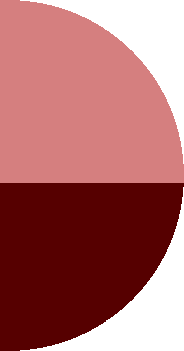
\includegraphics[scale=0.1]{resources/3/confusionCircleTN+FP}}$ & $= \frac{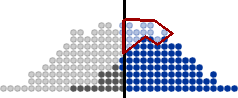
\includegraphics[scale=0.6]{resources/4/loanFP}}{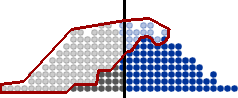
\includegraphics[scale=0.6]{resources/4/loanTN+FP}}$\\ \hline
\end{tabular}
\subsection{roc\_auc}
\begin{enumerate}
\item The \textbf{area under} the \textbf{curve} of the \textbf{ROC}-curve, a measure between 0.5 (worthless) and 1.0 (perfect: getting no FPs), rates the ability of a model to achieve a blend of recall and precision
\end{enumerate}
\begin{tabular}{|l|l|l|l|}
\hline
2. & 3. & 4.\\ 
- & -& - \\ \hline
\end{tabular}
\begin{description}
\item The receiver operating characteristic (ROC) curve plots the TPR versus FPR as a function of the model’s threshold for classifying a positive
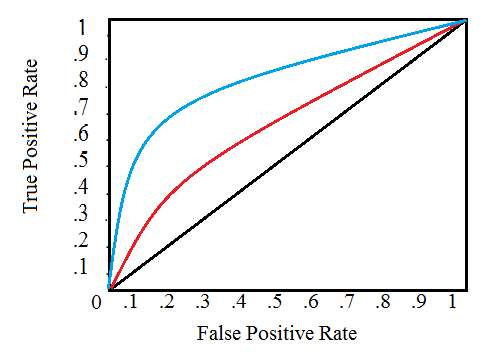
\includegraphics[scale=0.5]{resources/3/ROCcurve}
\item Increasing the threshold $\rightarrow$ moving up a curve ($\equiv$ model) to the top right corner, where all data is predicted as positive (threshold = 1.0) and vice versa
\end{description}
%
\subsection{pr\_auc}
(see: \href{http://www.chioka.in/differences-between-roc-auc-and-pr-auc/}{link 1} and \href{https://acutecaretesting.org/en/articles/precision-recall-curves-what-are-they-and-how-are-they-used}{link 2})
\begin{enumerate}
\item The \textbf{area under} the \textbf{curve} of the \textbf{PR}-curve, same: similar objective as the \textbf{roc\_auc}, but PR curves are better than ROC curves if the populations are imbalanced
\end{enumerate}
\begin{description}
\item The PR-curve plots the Precision versus the Recall 
\item 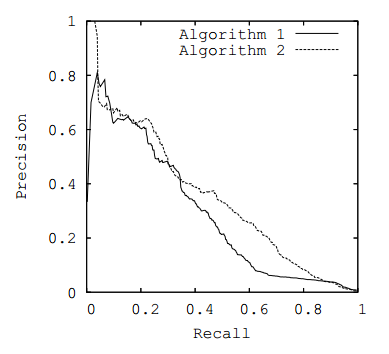
\includegraphics[scale=0.7]{resources/3/PRcurve}
\item Instead of the top left corner for the ROC-curve, here, we want to be in the top right corner for our classifier to be perfect
\end{description}
%
\subsection{accuracy}
\begin{enumerate}
\item Measuring the portion of correctly predicted data
\end{enumerate}
\begin{tabular}{|l|l|l|l|}
\hline
2. & 3. & 4.\\ 
$= \frac{\texttt{TP}+\texttt{TN}}{\texttt{Total}}$ & $= \frac{
\includegraphics[scale=0.1]{resources/3/confusionCircleTP+TN}}{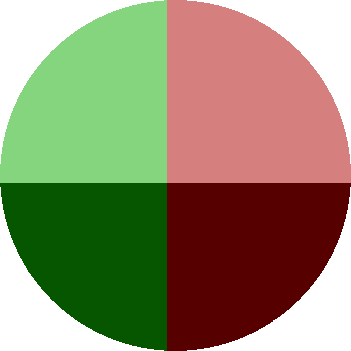
\includegraphics[scale=0.1]{resources/3/confusionCircleTotal}}$ & $= \frac{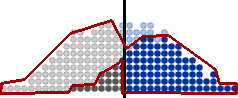
\includegraphics[scale=0.6]{resources/4/loanTP+TN}}{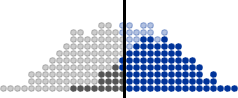
\includegraphics[scale=0.6]{resources/4/loanTotal}}$\\ \hline
\end{tabular}
\subsection{match\_rate}
\begin{enumerate}
\item The proportion of observations matched/not-matched
\end{enumerate}
\begin{tabular}{|l|l|l|l|}
\hline
2. & 3. & 4.\\ 
$= \frac{\texttt{TP}+\texttt{FP}}{\texttt{Total}}$ & $= \frac{
\includegraphics[scale=0.1]{resources/3/confusionCircleTP+FP}}{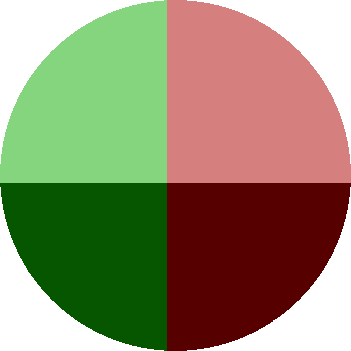
\includegraphics[scale=0.1]{resources/3/confusionCircleTotal}}$ & $= \frac{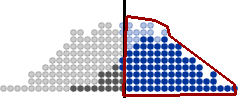
\includegraphics[scale=0.6]{resources/4/loanTP+FP}}{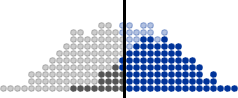
\includegraphics[scale=0.6]{resources/4/loanTotal}}$\\ \hline
\end{tabular}
%
\subsection{filter\_rate}
\begin{enumerate}
\item The proportion of observations filtered/not-filtered
\end{enumerate}
\begin{tabular}{|l|l|l|l|}
\hline
2. & 3. & 4.\\ 
$= 1-\texttt{match\_rate} = \frac{\texttt{TN}+\texttt{FN}}{\texttt{Total}} $ & $= \frac{
\includegraphics[scale=0.1]{resources/3/confusionCircleTN+FN}}{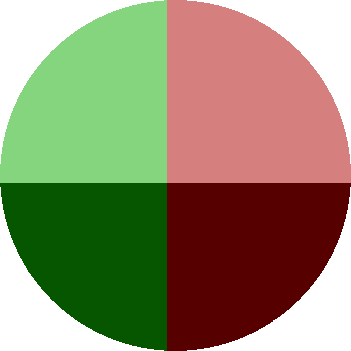
\includegraphics[scale=0.1]{resources/3/confusionCircleTotal}}$ & $= \frac{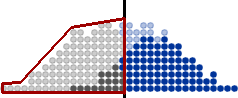
\includegraphics[scale=0.6]{resources/4/loanTN+FN}}{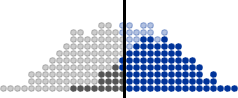
\includegraphics[scale=0.6]{resources/4/loanTotal}}$\\ \hline
\end{tabular}
%
\subsection{counts}
\begin{enumerate}
\item The number of edits labeled as \textit{false} and \textit{true}
\end{enumerate}
\begin{tabular}{|l|l|l|l|}
\hline
2. & 3. & 4.\\ 
- & - & - \\ \hline
\end{tabular}
\begin{description}
\item When calling the enwiki damaging model for example (\href{https://ores.wikimedia.org/v3/scores/enwiki/?models=damaging&model_info=statistics}{Link}), you'll notice the following under counts:
\item 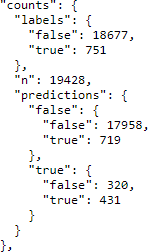
\includegraphics[scale=1]{resources/4/enwikiDamagingCounts}
\item The information stored in \textit{labels} is what we defined above under \textbf{1.}
\item \textit{n} is the total number of edits taken into account
\item \textit{predictions} is where it gets interesting: \textit{false} and \textit{true} as parents of another two of those are the labels and the values of their ``child''-booleans are the actual values of their edits
\item $\Rightarrow$ e.g. of 18677 edits that were labeled as \textit{false}, 719 were false negatives
\end{description}
%
\subsection{rates}
\begin{enumerate}
\item The rates simply equal $\frac{\texttt{label}}{\texttt{n}}$, both from \textbf{counts} for \textit{rates}: \textit{sample}: \textit{label}, and with \textit{label} = \textit{false} or \textit{true}
\begin{description}
\item So \textit{rates}: \textit{sample}: \textit{false}: $0.961 = \frac{18677}{19428}$  
\end{description}
\end{enumerate}
\begin{tabular}{|l|l|l|l|}
\hline
2. & 3. & 4.\\ 
- & - & - \\ \hline
\end{tabular}
\begin{description}
\item Calling the API the same way as for \textbf{counts}, we get:
\item 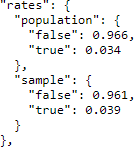
\includegraphics[scale=1]{resources/4/enwikiDamagingRates}
\item As already mentioned, the size of \textit{sample} equals our \textit{n} in \textbf{counts} $= 19428$.
\item But why have a sample and the whole population? Because there is a significant number of bot edits and edits that don't need reviewing (admins, autopatrolled users). The sample of edits does not contain any of those.
\end{description}
%
\subsection{!$<$metric$>$}
\begin{itemize}
\item Any $<$metric$>$ with an exclamation mark is the same metric for the negative class
\item e.g. recall $= \frac{\texttt{TP}}{\texttt{TP} + \texttt{FN}} \Rightarrow$ \textbf{!}recall  $= \frac{\texttt{TN}}{\texttt{TN} + \texttt{FP}}$
\item Example usage: find all items that are not ``E'' class $\rightarrow$ look at \textbf{!}recall for ``E'' class.
\end{itemize}
\subsubsection{Existing !$<$metric$>$s}
\begin{itemize}
\item !f1
\item !precision
\item !recall
\end{itemize}
%
\subsection{Additional explanations}
\subsubsection{recall vs precision}
When increasing one of these two, the other one naturally decreases. For an intuitive example, let's take a look at \href{https://research.google.com/bigpicture/attacking-discrimination-in-ml/}{Google's Loan Threshold Simulation}:\\
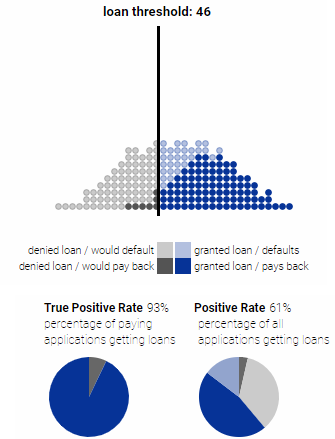
\includegraphics[scale=0.6]{resources/3/loanML3}\\
\begin{description}
\item The dark grey / dark blue dots, representing clients that would actually pay back their loan, are more and more included ($\rightarrow$ given loans) if we move the threshold further to the left.
\item But so are clients that would not. Thus moving the threshold to the left increases the \textbf{recall} (\textbf{tpr}) but decreases the \textbf{precision} and vice versa when moving to the right.
\end{description}
%
\subsubsection{roc\_auc vs pr\_auc}
see: \url{https://www.kaggle.com/general/7517}
\begin{itemize}
\item tl;dr: if the class imbalance problem exists, \textbf{pr\_auc} is more appropriate than \textbf{roc\_auc}
\begin{description}
\item If TNs are not meaningful to the problem or there are a lot more negatives than positives, \textbf{pr\_auc} is the way to go (it does not account for TNs).
\end{description}
\item In other words: 
\begin{itemize}
\item If the model needs to perform equally on the positive and negative class $\rightarrow$ \textbf{roc\_auc}
\item If it's not interesting how the model performs on negative class $\rightarrow$ \textbf{pr\_auc} (example: detecting cancer; find all positives and make sure they're correct!)
\end{itemize}
\end{itemize}
%
%
%
%
\section*{Questions}
\begin{itemize}
%
\item \colorbox{yellow}{Q:} Should I ask Aaron how he would like us to work together? I'm not sure how he meant it.
\begin{description}
\item \colorbox{orange}{A:} 
\end{description}
%
\item \colorbox{yellow}{Q:} In what situations exactly do we want to optimize the threshold in the context of user centered threshold optimization?
\begin{description}
\item \colorbox{orange}{A:} 
\end{description}
%
\end{itemize}
\end{document}